% rubber: set program xelatex
%%%%%%%%%%%%%%%%%%%%%%%%%%%%%%%%%%%%%%%
% Deedy - One Page Two Column Resume
% LaTeX Template
% Version 1.2 (16/9/2014)
%
% Original author:
% Debarghya Das (http://debarghyadas.com)
%
% Original repository:
% https://github.com/deedydas/Deedy-Resume
%
% IMPORTANT: THIS TEMPLATE NEEDS TO BE COMPILED WITH XeLaTeX
%
% This template uses several fonts not included with Windows/Linux by
% default. If you get compilation errors saying a font is missing, find the line
% on which the font is used and either change it to a font included with your
% operating system or comment the line out to use the default font.
% 
%%%%%%%%%%%%%%%%%%%%%%%%%%%%%%%%%%%%%%
% 
% TODO:
% 1. Integrate biber/bibtex for article citation under publications.
% 2. Figure out a smoother way for the document to flow onto the next page.
% 3. Add styling information for a "Projects/Hacks" section.
% 4. Add location/address information
% 5. Merge OpenFont and MacFonts as a single sty with options.
% 
%%%%%%%%%%%%%%%%%%%%%%%%%%%%%%%%%%%%%%
%
% CHANGELOG:
% v1.1:
% 1. Fixed several compilation bugs with \renewcommand
% 2. Got Open-source fonts (Windows/Linux support)
% 3. Added Last Updated
% 4. Move Title styling into .sty
% 5. Commented .sty file.
%
%%%%%%%%%%%%%%%%%%%%%%%%%%%%%%%%%%%%%%%
%
% Known Issues:
% 1. Overflows onto second page if any column's contents are more than the
% vertical limit
% 2. Hacky space on the first bullet point on the second column.
%
%%%%%%%%%%%%%%%%%%%%%%%%%%%%%%%%%%%%%%


\documentclass[]{deedy-resume-openfont}
\usepackage{fancyhdr}

\usepackage[dvips,xetex]{graphicx}
% \usepackage{ifpdf,mla}
 
\pagestyle{fancy}
\fancyhf{}
 
\begin{document}

%%%%%%%%%%%%%%%%%%%%%%%%%%%%%%%%%%%%%%
%
%     LAST UPDATED DATE
%
%%%%%%%%%%%%%%%%%%%%%%%%%%%%%%%%%%%%%%
\lastupdated

%%%%%%%%%%%%%%%%%%%%%%%%%%%%%%%%%%%%%%
%
%     TITLE NAME
%
%%%%%%%%%%%%%%%%%%%%%%%%%%%%%%%%%%%%%%
\namesection{Stefan}{Matting}{
    \href{mailto:stefan.matting@gmail.com.com}{stefan.matting@gmail.com} | +4917625558115
    % \urlstyle{same}\href{http://debarghyadas.com}{debarghyadas.com}| \href{http://fb.co/dd}{fb.co/dd}\\
    % \href{mailto:deedy@fb.com}{deedy@fb.com} | 607.379.5733 | \href{mailto:dd367@cornell.edu}{dd367@cornell.edu}
}

%%%%%%%%%%%%%%%%%%%%%%%%%%%%%%%%%%%%%%
%
%     COLUMN ONE
%
%%%%%%%%%%%%%%%%%%%%%%%%%%%%%%%%%%%%%%

\begin{minipage}[t]{0.33\textwidth} 

%%%%%%%%%%%%%%%%%%%%%%%%%%%%%%%%%%%%%%
%     LINKS
%%%%%%%%%%%%%%%%%%%%%%%%%%%%%%%%%%%%%%


\section{About} 

\begin{center}
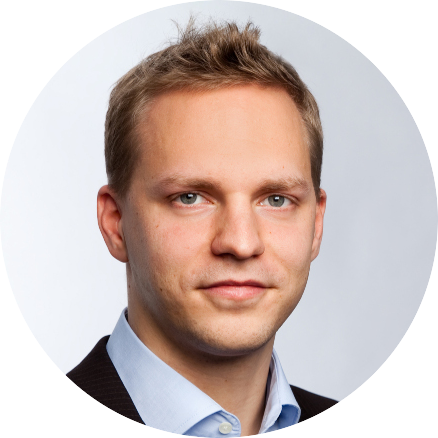
\includegraphics[scale=0.3]{mug-round.png}
\end{center}

GitHub: \href{https://github.com/smatting}{\bf smatting} \\
LinkedIn:  \href{https://www.linkedin.com/in/stefanmatting/}{\bf stefanmatting} \\
Hobbies: making music \textbullet{} hacking

%%%%%%%%%%%%%%%%%%%%%%%%%%%%%%%%%%%%%%
%     SKILLS
%%%%%%%%%%%%%%%%%%%%%%%%%%%%%%%%%%%%%%



\sectionsep
\section{Skills}

\sectionsep
\subsection{Data Science}
\textbullet{} Analysis (all Python data tools) \\
\textbullet{} Machine Learning (scikit-learn, xgboost) \\
\textbullet{} Deep Learning (pytorch, tensorflow) \\
\textbullet{} Bayesian Statistical Modelling (Stan)\\

\sectionsep
\subsection{Data Engineering}
    \textbullet{} ETL (Python + SQL) \\
    \textbullet{} Import / Export with external APIs \\
    \textbullet{} Logfile parsing \\
    \textbullet{} Data Stream Processing (Python + RabbitMQ) \\
    \textbullet{} PostgreSQL \\
    \textbullet{} MongoDB \\
    \textbullet{} ElasticSearch \\

\sectionsep
\subsection{Development}
    \textbullet{} Python (7+ years)  \\
    \textbullet{} Haskell \\
    \textbullet{} git + CI/CD workflows \\
    \textbullet{} Javascript/Elm/React/Vue.js \\

\sectionsep
\subsection{Operations}
    \textbullet{} GNU/Linux \\
    \textbullet{} systemd \\
    \textbullet{} AWS / Telekom Cloud \\
    \textbullet{} filebeat + logstash + ELK \\
    \textbullet{} salt \\
    \textbullet{} nixos + nixops \\
    \textbullet{} Docker \\
   
\sectionsep
\subsection{Languages}
German (fluent) \textbullet{}
English (fluent) \textbullet{}
French



%%%%%%%%%%%%%%%%%%%%%%%%%%%%%%%%%%%%%%
%
%     COLUMN TWO
%
%%%%%%%%%%%%%%%%%%%%%%%%%%%%%%%%%%%%%%

\end{minipage} 
\hfill
\begin{minipage}[t]{0.62\textwidth} 

%%%%%%%%%%%%%%%%%%%%%%%%%%%%%%%%%%%%%%
%     EXPERIENCE
%%%%%%%%%%%%%%%%%%%%%%%%%%%%%%%%%%%%%%

\section{Experience}

\runsubsection{AskBy GmBH}
\descript{| ML Developer }
\location{Apr 2018 - Present | Berlin}
\vspace{10pt} % Hacky fix for awkward extra vertical space

At AskBy I\ldots
\vspace{9pt} % Hacky fix for awkward extra vertical space
\begin{tightemize}
\item manage AskBy's operations and infrastructure
\item developed the Backend of the AskBy NLQuery App -- a chat interface for Webtrekk's users.
    Quality is assured via: a scalable by service-oriented design, application logging, monitoring and alerting, domain event streaming, ETL to PostgreSQL for analysis
\item research and develop solutions that are powered by Natural Language Processing algorithms
\end{tightemize}
\sectionsep

\runsubsection{Outfittery GmbH}
\descript{| Machine Learning Specialist }
\location{Dec 2013 - Dec 2017 | Berlin}
\vspace{10pt} % Hacky fix for awkward extra vertical space
At Outfittery I\ldots
\vspace{3pt} % Hacky fix for awkward extra vertical space
\begin{tightemize}
% \item Hired as the first data scientist and helped in building the data department for 4 years
\item lead a small team of data scientists. We autonomously developed solutions all the way from initial research to live production systems
\item designed and developed the platform that integrates all algorithms from the data science team into the IT system
\item built a diagnostic tool that connects applications failure log events (ElasticSearch) with Web Tracking Data (Snowplow)
\item optimized the steering of several business processes with predictive Machine Learning models
% \item Increased the efficiency of Outfittery's stylists by developing several data products in the fashion domain: item matching, visual similarity of items, customer-based item recommendation, outfit search
% \item Developed a business forecast model based on a Markov chain model
% \item Estimated customer behaviour with various ML models
% \item Migrated all customer and article data between systems
\end{tightemize}
\sectionsep


\runsubsection{Fraunhofer-Institut für Solare Energiesysteme}
\descript{| Research assistant }
\location{Mar 2008 - Feb 2013 | Freiburg im Breisgau}
\begin{tightemize}
\item Research assistant to Dr. Simon Schwunk
\item Assisted in developing algorithms that estimate that internal state of several battery types
\item Developed a modular simulation software for photovoltaic systems
\item Ported multiple algorithms to embedded systems
\end{tightemize}
\sectionsep


\runsubsection{Universitäts-Klinikum Freiburg}
\descript{| Research assistant }
\location{Jun 2010 - Nov 2010 | Freiburg im Breisgau}
\begin{tightemize}
\item Research assistant to Prof. Dr. Thilo Hinterberger
\item Assisted in developing software system that evaluates EEG measurements
\end{tightemize}
\sectionsep

%%%%%%%%%%%%%%%%%%%%%%%%%%%%%%%%%%%%%%
%     EDUCATION
%%%%%%%%%%%%%%%%%%%%%%%%%%%%%%%%%%%%%%

\section{Education} 

\subsection{Albert-Ludwigs-Universität Freiburg}
\descript{Mathematics and Computer Science studies}
\location{2005 - 2013 | Freiburg im Breigau}
Gradudated with a "Diplom Mathematik" with a final grade of 1.0 with my thesis on ``Preferential Attachment Modell und Verzweigungsprozesse''

\sectionsep
\subsection{Robert-Bosch Gymnasium}
\location{1991 - 2004 | Wendlingen, BW}
\sectionsep

%%%%%%%%%%%%%%%%%%%%%%%%%%%%%%%%%%%%%%
%     COURSEWORK
%%%%%%%%%%%%%%%%%%%%%%%%%%%%%%%%%%%%%%

% \section{Coursework}
% \subsection{Graduate}
% Advanced Machine Learning \\
% Open Source Software Engineering \\
% Advanced Interactive Graphics \\
% Compilers + Practicum \\
% Cloud Computing \\
% Evolutionary Computation \\
% Defending Computer Networks \\
% Machine Learning \\
% \sectionsep

% \subsection{Undergraduate}
% Information Retrieval \\
% Operating Systems \\
% Artificial Intelligence + Practicum \\
% Functional Programming \\
% Computer Graphics + Practicum \\
% {\footnotesize \textit{\textbf{(Research Asst. \& Teaching Asst 2x) }}} \\
% Unix Tools and Scripting \\


%%%%%%%%%%%%%%%%%%%%%%%%%%%%%%%%%%%%%%
%     RESEARCH
%%%%%%%%%%%%%%%%%%%%%%%%%%%%%%%%%%%%%%

% \section{Research}
% \runsubsection{Cornell Robot Learning Lab}
% \descript{| Researcher}
% \location{Jan 2014 – Jan 2015 | Ithaca, NY}
% Worked with \textbf{\href{http://www.cs.cornell.edu/~ashesh/}{Ashesh Jain}} and \textbf{\href{http://www.cs.cornell.edu/~asaxena/}{Prof Ashutosh Saxena}} to create \textbf{PlanIt}, a tool which  learns from large scale user preference feedback to plan robot trajectories in human environments.  
% \sectionsep

% \runsubsection{Cornell Phonetics Lab}
% \descript{| Head Undergraduate Researcher}
% \location{Mar 2012 – May 2013 | Ithaca, NY}
% Led the development of \textbf{QuickTongue}, the first ever breakthrough tongue-controlled game with \textbf{\href{http://conf.ling.cornell.edu/~tilsen/}{Prof Sam Tilsen}} to aid in Linguistics research. 
% \sectionsep

%%%%%%%%%%%%%%%%%%%%%%%%%%%%%%%%%%%%%%
%     AWARDS
%%%%%%%%%%%%%%%%%%%%%%%%%%%%%%%%%%%%%%

% \section{Awards} 
% \begin{tabular}{rll}
% 2014	     & top 52/2500  & KPCB Engineering Fellow\\
% 2014	     & 1\textsuperscript{st}/50  & Microsoft Coding Competition, Cornell\\
% 2013	     & National  & Jump Trading Challenge Finalist\\
% 2013     & 7\textsuperscript{th}/120 & CS 3410 Cache Race Bot Tournament  \\
% 2012     & 2\textsuperscript{nd}/150 & CS 3110 Biannual Intra-Class Bot Tournament \\
% 2011     & National & Indian National Mathematics Olympiad (INMO) Finalist \\
% \end{tabular}
% \sectionsep

%%%%%%%%%%%%%%%%%%%%%%%%%%%%%%%%%%%%%%
%     PUBLICATIONS
%%%%%%%%%%%%%%%%%%%%%%%%%%%%%%%%%%%%%%

% \section{Publications} 
% \renewcommand\refname{\vskip -1.5cm} % Couldn't get this working from the .cls file
% \bibliographystyle{abbrv}
% \bibliography{publications}
% \nocite{*}

\end{minipage} 
\end{document}  \documentclass[]{article}
